\usepackage{stmaryrd}%! Author = zero
%! Date = 29/07/2024

\documentclass[a4paper, 12pt]{article}

\usepackage[english,russian]{babel}
\usepackage[T2A]{fontenc}
\usepackage[utf8]{inputenc}
\usepackage{geometry}
\usepackage{enumitem}
\usepackage{setspace}
\usepackage{amssymb}
\usepackage{graphicx}
\usepackage{float}
\usepackage{wrapfig}
\geometry{top=5mm}
\renewcommand{\arraystretch}{1.2}
\linespread{1}

% Document
\begin{document}
    \begin{center}
        \textbf{Задачи №5 Решение задач}\\
    \end{center}

    \begin{center}
        \textbf{ЕГЭ}\\
    \end{center}

    \begin{enumerate}
        \begin{spacing}{1.2}
            \item Введем обозначения:\\
            $(x \in P) = P, (x \in Q) = Q, (x \in A) = A$\\
            Преобразуем выражение:\\
            $(P \leftrightarrow Q) \rightarrow \bar A = $
            $\overline{(P \leftrightarrow Q)} \vee \bar A = $
            $\overline{(P \wedge Q \vee \bar P \wedge \bar Q)} \vee \bar A = $\\
            $(\bar P \vee \bar Q) \wedge (P \vee Q) \vee \bar A = $
            $\bar P \wedge Q \vee P \wedge \bar Q \vee \bar A$\\
            Заметим, что $\bar P \wedge Q = 1$ не имеет решения, \\а $P \wedge \bar Q = 1$ при $x \in [25; 32) \cup (47; 50]$.\\
            Следовательно, чтобы выражение было истинным при любом $x$: \\
            $\bar A \in (-\infty; 25) \cup [32; 47] \cup [50; +\infty]$, тогда \\
            $A \in [25; 32)$ или $A \in (47; 50]$\\
            $32 - 25 = 7$ или $50 - 47 = 3$\\
            Ответ: 7
            \begin{figure}[h]
                \centering
                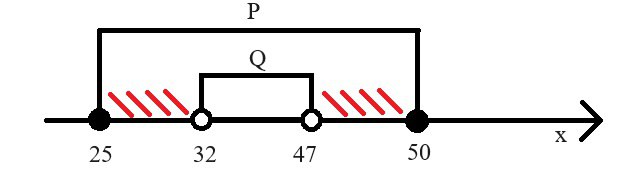
\includegraphics[width=0.5  \linewidth]{images/img}
            \end{figure}

            \item Введем обозначения:\\
            $(x \in P) = P, (x \in Q) = Q, (x \in A) = A$\\
            Преобразуем выражение:\\
            $(\bar A \rightarrow P) \rightarrow (A \rightarrow Q) = $
            $\overline{A \vee P} \vee \bar A \vee Q = $
            $\bar A \wedge \bar P \vee \bar A \vee Q = $
            $\bar A \vee Q$\\
            Заметим, что $Q = 1$ при $x \in [14; 23]$.\\
            Следовательно, чтобы выражение было истинным при любом $x$: \\
            $\bar A \in (-\infty; 14) \cup (23; +\infty)$, тогда \\
            $A \in [14; 23]$ \\
            $23 - 14 = 9$\\
            Ответ: 9
            \begin{figure}[h]
                \centering
                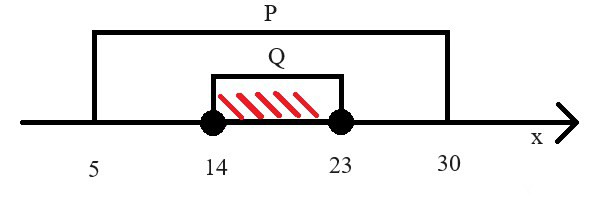
\includegraphics[width=0.5  \linewidth]{images/img_1}
            \end{figure}

            \item Введем обозначения:\\
            $(x \in P) = P, (x \in Q) = Q, (x \in A) = A$\\
            Преобразуем выражение:\\
            $(P \wedge Q) \rightarrow A = $
            $\bar P \vee \bar Q \vee A$\\
            Заметим, что $\bar P \vee \bar Q = 1$ при $x \in (-\infty; 12) \cup (15; +\infty)$.\\
            Следовательно, чтобы выражение было истинным при любом $x$: \\
            $A \in [12; 15]$\\
            $15 - 12 = 3$\\
            Ответ: 3
            \begin{figure}[h]
                \centering
                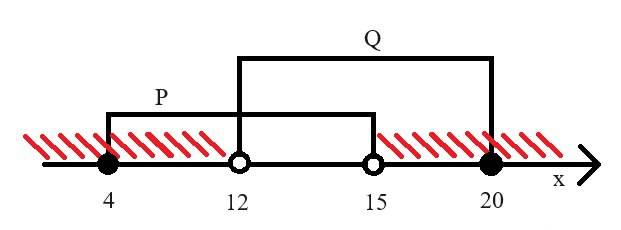
\includegraphics[width=0.5  \linewidth]{images/img_2}
            \end{figure}

            \item Введем обозначения:\\
            $(x \in P) = P, (x \in Q) = Q, (x \in R) = R, (x \in A) = A$\\
            Преобразуем выражение:\\
            $(A \vee P) \vee (Q \rightarrow R) = $
            $A \vee P \vee \bar Q \vee R$\\
            Заметим, что $P \vee \bar Q \vee R = 1$ при $x \in (-\infty; 5) \cup [10; +\infty)$.\\
            Следовательно, чтобы выражение было истинным при любом $x$: \\
            $A \in [5; 10)$, тогда \\
            $10 - 5 = 5$\\
            Ответ: 5
            \begin{figure}[h]
                \centering
                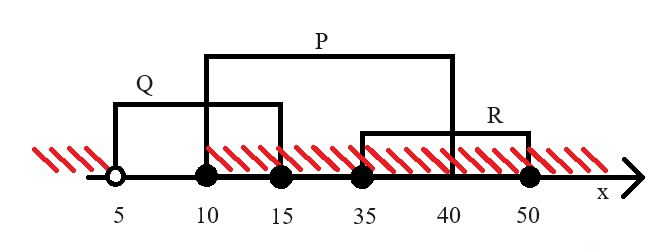
\includegraphics[width=0.5  \linewidth]{images/img_3}
            \end{figure}

            \item Введем обозначения:\\
            $(x \in P) = P, (x \in Q) = Q, (x \in R) = R, (x \in A) = A$\\
            Преобразуем выражения:\\
            $Q \rightarrow R = \bar Q \vee R$\\
            $A \rightarrow P = \bar A \vee P$\\
            Заметим, что в первом выражении $\bar Q \vee R = 1$ при $x \in (-\infty; 15] \cup (20; +\infty)$.\\
            Во втором выражении $P = 1$ при $x \in [10; 15]$.\\
            Следовательно, чтобы выражения принимали одинаковые значения при любом $x$:\\
            $\bar A \in (-\infty; 15] \cup (20; +\infty)$, тогда \\
            $A \in (15; 20]$
            $20 - 15= 5$\\
            Ответ: 5
            \begin{figure}[h]
                \centering
                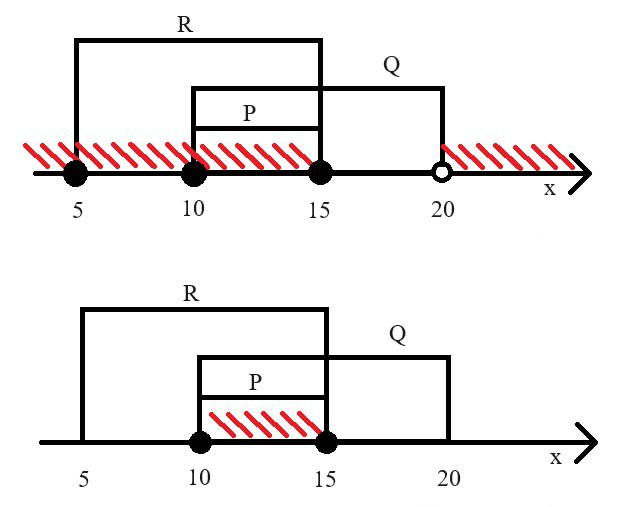
\includegraphics[width=0.5  \linewidth]{images/img_4}
            \end{figure}\\

            \newpage
            \item Введем обозначения:\\
            $(x \in P) = P, (x \in Q) = Q, (x \in A) = A$\\
            Преобразуем выражения:\\
            $\bar A \rightarrow \bar P = A \vee \bar P$\\
            $Q \rightarrow A = \bar Q \vee A$\\
            Заметим, что в первом выражении $\bar P = 1$ при $x \in (-\infty; 30) \cup (45; +\infty)$, тогда\\
            чтобы выражение было истинным при любом $x$, $A \in [30; 45]$\\
            Во втором выражении $\bar Q = 1$ при $x \in (-\infty; 40) \cup (55; +\infty)$, тогда\\
            чтобы выражение было истинным при любом $x$, $A \in [40; 55]$\\
            Следовательно, чтобы оба выражения принимали истинные значения при любом $x$:\\
            $A \in [30; 55]$
            $55 - 30 = 25$\\
            Ответ: 25
            \begin{figure}[h]
                \centering
                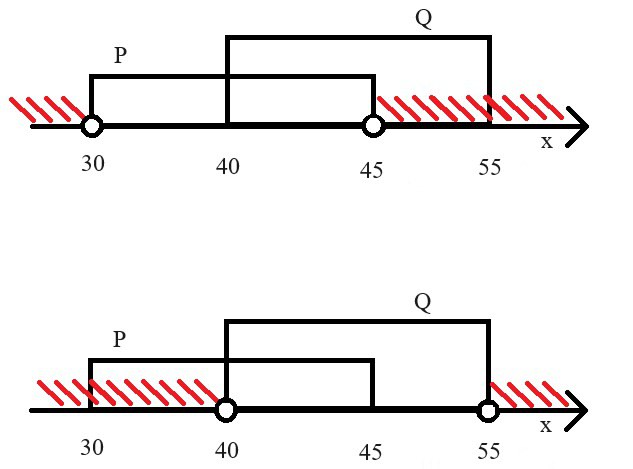
\includegraphics[width=0.5  \linewidth]{images/img_5}
            \end{figure}


        \end{spacing}
    \end{enumerate}

    \newpage
    \begin{center}
        \textbf{Открытая олимпиада школьников по информатике ИТМО}
    \end{center}

    \begin{center}
        \textbf{№1 Сплошные следования}
    \end{center}

    \begin{enumerate}
        \item $(x \rightarrow y) \leftrightarrow z = 1 \leftrightarrow z = z$

        \item $((x \wedge \overline y) \leftrightarrow (y \wedge z)) \rightarrow (y \leftrightarrow z) = $
        $(0 \leftrightarrow 0) \rightarrow (0) = 0$

        \item $(x \rightarrow y) \rightarrow (y \oplus z) = 1 \rightarrow (\bar y \wedge z \vee y \wedge \bar z) = 1$

        \item $(\overline{z \oplus y}) \rightarrow (y \rightarrow z) = $
        $\overline{\bar z \wedge y \vee z \wedge \bar y} \rightarrow (\bar y \vee z) = $
        $0 \rightarrow 1$  или $0 \rightarrow 0= 1$

        \item $(\overline y \wedge z) \rightarrow (y \leftrightarrow \overline x) = $
        $y \vee \bar z \vee \bar x \wedge y \vee x \wedge \bar y$
    \end{enumerate}
    Ответ: 2, 3, 4

    \begin{center}
        \textbf{№2 Затухание}
    \end{center}

    \begin{figure}[h]
        \centering
        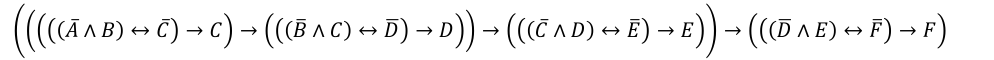
\includegraphics[width=1.2  \linewidth]{images/im1}
    \end{figure}

    Решим по действиям:
    \begin{enumerate}
        \begin{spacing}{1.5}
            \item $((\bar A \wedge B) \leftrightarrow \bar C) \rightarrow C = $
            $\bar A \wedge B \wedge \bar C \vee (A \vee \bar B) \wedge C \rightarrow C = $\\
            $\bar A \wedge B \wedge \bar C \vee A \wedge C \vee \bar B \wedge C \rightarrow C = $
            $(A \vee \bar B \vee C) \wedge (\bar A \vee \bar C) \wedge (B \vee \bar C) \vee C = $\\
            $(A \wedge \bar C \vee \bar A \wedge \bar B \vee \bar B \wedge \bar C \vee \bar A \wedge C) \wedge (B \vee \bar C) \vee C = $\\
            $A \wedge B \wedge \bar C \vee A \wedge \bar C \vee \bar A \wedge \bar B \wedge \bar C \vee \bar B \wedge \bar C \vee \bar A \wedge B \wedge C \vee C = $
            $A \wedge \bar C \vee \bar B \wedge \bar C \vee C$

            \item $((\bar B \wedge C) \leftrightarrow \bar D) \rightarrow D = $
            $\bar B \wedge C \wedge \bar D \vee (B \vee \bar C) \wedge D \rightarrow D = $\\
            $\bar B \wedge C \wedge \bar D \vee B \wedge D \vee \bar C \wedge D \rightarrow D = $
            $(B \vee \bar C \vee D) \wedge (\bar B \vee \bar D) \wedge (C \vee \bar D) \vee D = $\\
            $(B \wedge \bar D \vee \bar B \wedge \bar C \vee \bar C \wedge \bar D \vee \bar B \wedge D) \wedge (C \vee \bar D) \vee D = $\\
            $B \wedge C \wedge \bar D \vee B \wedge \bar D \vee \bar B \wedge \bar C \wedge \bar D \vee \bar C \wedge \bar D \vee \bar B \wedge C \wedge D \vee D = $
            $B \wedge \bar D \vee \bar C \wedge \bar D \vee D$

            \item $((\bar C \wedge D) \leftrightarrow \bar E) \rightarrow E) = $
            $\bar C \wedge D \wedge \bar E \vee (C \vee \bar D) \wedge E \rightarrow E = $\\
            $\bar C \wedge D \wedge \bar E \vee C \wedge E \vee \bar D \wedge E \rightarrow E = $
            $(C \vee \bar D \vee E) \wedge (\bar C \vee \bar E) \wedge (D \vee \bar E) \vee E = $\\
            $(C \wedge \bar E \vee \bar C \wedge \bar D \vee \bar D \wedge \bar E \vee \bar C \wedge E) \wedge (D \vee \bar E) \vee E = $\\
            $C \wedge D \wedge \bar E \vee C \wedge \bar E \vee \bar C \wedge \bar D \wedge \bar E \vee \bar D \wedge \bar E \vee \bar C \wedge D \wedge E \vee E = $
            $C \wedge \bar E \vee \bar D \wedge \bar E \vee E$

            \item $((\bar D \wedge E) \leftrightarrow \bar F) \rightarrow F = $
            $\bar D \wedge E \wedge \bar F \vee (D \vee \bar E) \wedge F \rightarrow F = $\\
            $\bar D \wedge E \wedge \bar F \vee D \wedge F \vee \bar E \wedge F \rightarrow F = $
            $(D \vee \bar E \vee F) \wedge (\bar D \vee \bar F) \wedge (E \vee \bar F) \vee F = $\\
            $(D \wedge \bar F \vee \bar D \wedge \bar E \vee \bar E \wedge \bar F \vee \bar D \wedge F) \wedge (E \vee \bar F) \vee F = $\\
            $D \wedge E \wedge \bar F \vee D \wedge \bar F \vee \bar D \wedge \bar E \wedge \bar F \vee \bar E \wedge \bar F \vee \bar D \wedge E \wedge F \vee F = $
            $D \wedge \bar F \vee \bar E \wedge \bar F \vee F$

            \item $A \wedge \bar C \vee \bar B \wedge \bar C \vee C \rightarrow B \wedge \bar D \vee \bar C \wedge \bar D \vee D = $\\
            $(\bar A \vee C) \wedge (B \vee C) \wedge \bar C \vee B \wedge \bar D \vee \bar C \wedge \bar D \vee D = $\\
            $(\bar A \wedge B \vee \bar A \wedge C \vee B \wedge C \vee C) \wedge \bar C \vee B \wedge \bar D \vee \bar C \wedge \bar D \vee D = $
            $\bar A \wedge B \wedge \bar C \vee B \wedge \bar D \vee \bar C \wedge \bar D \vee D$

            \item $\bar A \wedge B \wedge \bar C \vee B \wedge \bar D \vee \bar C \wedge \bar D \vee D \rightarrow C \wedge \bar E \vee \bar D \wedge \bar E \vee E = $\\
            $(A \vee \bar B \vee C) \wedge (\bar B \vee D) \wedge (C \vee D) \wedge \bar D \vee C \wedge \bar E \vee \bar D \wedge \bar E \vee E = $\\
            $(A \wedge \bar B \vee A \wedge D \vee \bar B \vee \bar B \wedge D \vee \bar B \wedge C \vee C \wedge D) \wedge (C \vee D) \wedge \bar D \vee C \wedge \bar E \vee \bar D \wedge \bar E \vee E = $
            $(\bar B \vee A \wedge D \vee C \wedge D) \wedge C \wedge \bar D \vee C \wedge \bar E \vee \bar D \wedge \bar E \vee E = $
            $\bar B \wedge C \wedge \bar D \vee C \wedge \bar E \vee \bar D \wedge \bar E \vee E$

            \item $\bar B \wedge C \wedge \bar D \vee C \wedge \bar E \vee \bar D \wedge \bar E \vee E \rightarrow D \wedge \bar F \vee \bar E \wedge \bar F \vee F = $\\
            $(B \vee \bar C \vee D) \wedge (\bar C \vee E) \wedge (D \vee E) \wedge \bar E \vee D \wedge \bar F \vee \bar E \wedge \bar F \vee F = $\\
            $(B \wedge \bar C \vee B \wedge E \vee \bar C \vee \bar C \wedge E \vee D \wedge \bar C \vee D \wedge E) \wedge \bar E \wedge D \vee D \wedge \bar F \vee \bar E \wedge \bar F \vee F = $
            $(\bar C \vee B \wedge E \vee D \wedge E) \wedge \bar E \wedge D \vee D \wedge \bar F \vee \bar E \wedge \bar F \vee F = $
            $\bar C \wedge \bar E \wedge D \vee D \wedge \bar F \vee \bar E \wedge \bar F \vee F = $
            $\bar C \wedge \bar E \wedge D \vee D \wedge \bar F \vee \bar E \vee F = $
            $D \wedge \bar F \vee F \vee \bar E =$
            $D \vee F \vee \bar E$


        \end{spacing}
    \end{enumerate}


    \begin{center}
        \textbf{№3 Полусумматоры}
    \end{center}

    Составим уравнение:\\
    $x_1 \oplus \bar x_2 \vee x_2 \wedge x_3 \vee (x_2 \oplus \bar x_3) \wedge x_3 \wedge \bar x_4 \vee (x_3 \oplus \bar x_4) \vee x_4 \wedge \bar x_1 \vee x_1 \wedge \bar x_2 \wedge (x_4 \oplus \bar x_1) = 0$\\
    $x_1 \oplus \bar x_2 \vee x_2 \wedge x_3 \vee (\bar x_2 \wedge \bar x_3 \vee x_2 \wedge x_3) \wedge x_3 \wedge \bar x_4 \vee (x_3 \oplus \bar x_4) \vee x_4 \wedge \bar x_1 \vee x_1 \wedge \bar x_2 \wedge (x_4 \oplus \bar x_1) = 0$\\
    $x_1 \oplus \bar x_2 \vee x_2 \wedge x_3 \vee x_2 \wedge x_3 \wedge \bar x_4 \vee (x_3 \oplus \bar x_4) \vee x_4 \wedge \bar x_1 \vee x_1 \wedge \bar x_2 \wedge (x_4 \oplus \bar x_1) = 0$\\
    $x_1 \oplus \bar x_2 \vee x_2 \wedge x_3 \vee (x_3 \oplus \bar x_4) \vee x_4 \wedge \bar x_1 \vee x_1 \wedge \bar x_2 \wedge (\bar x_4 \wedge \bar x_1 \vee x_4 \wedge x_1) = 0$\\
    $x_1 \oplus \bar x_2 \vee x_2 \wedge x_3 \vee (x_3 \oplus \bar x_4) \vee x_4 \wedge \bar x_1 \vee x_1 \wedge \bar x_2 \wedge x_4 = 0$\\
    $x_1 \oplus \bar x_2 \vee x_2 \wedge x_3 \vee (x_3 \oplus \bar x_4) \vee x_4 \wedge(\bar x_1 \vee x_1 \wedge \bar x_2) = 0$\\
    $x_1 \oplus \bar x_2 \vee x_2 \wedge x_3 \vee (x_3 \oplus \bar x_4) \vee x_4 \wedge(\bar x_1 \vee \bar x_2) = 0$\\
    $\bar x_1 \wedge \bar x_2 \vee x_1 \wedge x_2 \vee x_2 \wedge x_3 \vee \bar x_3 \wedge \bar x_4 \vee x_3 \wedge x_4 \vee x_4 \wedge \bar x_1 \vee x_4 \wedge \bar x_2 = 0$

    \[
        \begin{cases}
            \bar x_1 \wedge \bar x_2 = 0
            \\
            x_1 \wedge x_2 = 0
            \\
            x_2 \wedge x_3 = 0
            \\
            \bar x_3 \wedge \bar x_4 = 0
            \\
            x_3 \wedge  x_4 = 0
            \\
            x_4 \wedge \bar x_1 = 0
            \\
            x_4 \wedge \bar x_2 = 0
        \end{cases}
        \rightarrow
        \begin{cases}
            x_1,  x_2 = {(1; 1), (1; 0), (0; 1)}
            \\
            x_1, x_2 = {(0; 0), (1; 0), (0; 1)}
            \\
            x_2, x_3 = {(0; 0), (1; 0), (0; 1)}
            \\
            x_3,  x_4 = {(1; 1), (1; 0), (0; 1)}
            \\
            x_3, x_4 = {(0; 0), (1; 0), (0; 1)}
            \\
            x_4,  x_1 = {(0; 1), (0; 0), (1; 1)}
            \\
            x_4,  x_2 = {(0; 1), (0; 0), (1; 1)}
        \end{cases}
        \rightarrow
        \begin{cases}
            x_1,  x_2 = {(1; 0), (0; 1)}
            \\
            x_2, x_3 = {(0; 0), (1; 0), (0; 1)}
            \\
            x_3,  x_4 = {(1; 0), (0; 1)}
            \\
            x_4,  x_1 = {(0; 1), (0; 0), (1; 1)}
            \\
            x_4,  x_2 = {(0; 1), (0; 0), (1; 1)}
        \end{cases}

    \]
    Пусть $x_1 = 1, x_2 = 0$, тогда $x_3 = 1, x_4 = 0$\\
    Пусть $x_1 = 0, x_2 = 1$, тогда решений нет\\
    Ответ: 1010


\end{document}